\documentclass[12pt, oneside]{book}
 
\usepackage{graphicx}
\usepackage[cmex10]{amsmath}
\usepackage{algorithmic}
\begin{document}
 
%titlepage
\thispagestyle{empty}
\begin{center}
\begin{minipage}{0.75\linewidth}
    \centering
%University logo
    %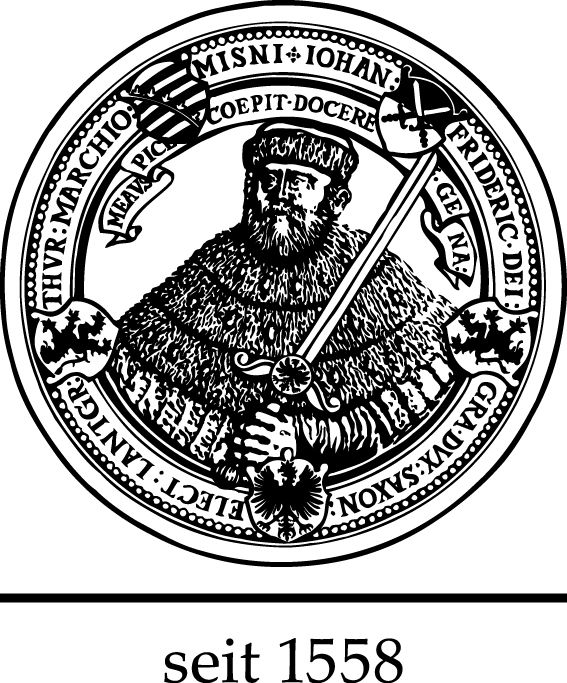
\includegraphics[width=0.3\linewidth]{logo.pdf}
    \rule{0.4\linewidth}{0.15\linewidth}\par
    \vspace{3cm}
%Thesis title
    {\uppercase{\Large the title of my thesis project which may span multiple lines\par}}
    \vspace{3cm}
%Author's name
    {\Large Mohammad Ali Rostami\par}
    \vspace{3cm}
%Degree
    {\Large Supervisor: Prof. Martin B{\"u}cker\par}
    
    \vspace{3cm}
%Date
    {\Large May 2014}
\end{minipage}
\end{center}
\clearpage

\newpage
\section*{Abstract}

\thispagestyle{empty}

\newpage
\section*{Acknowledgments}
\thispagestyle{empty}


\tableofcontents

\chapter{Introduction}
\chapter{Preliminaries}
%%%%%%%%%%%%%%%%%%%%%%%%%%%%%%%%%%%%%%%%%%%%%%%%%
%%%% SHEMAT
%%%%%%%%%%%%%%%%%%%%%%%%%%%%%%%%%%%%%%%%%%%%%%%%%
\section{SHEMAT}
We consider numerical simulations representing concrete problems arising from geothermal reservoir
engineering. To this end, a geothermal software package is currently being developed at the
Institute for Applied Geophysics and Geothermal Energy, E.ON Energy Research Center, at RWTH Aachen
University. This software is called Simulator for HEat and MAss Transport
(SHEMAT)~\cite{shemat,inverse-shemat}. 
It is capable of solving forward problems arising from fluid flow
in geothermal reservoirs. In SHEMAT, a forward problem consists of the coupled transient equations
for groundwater flow, heat transport, and the transport of reactive solutes in porous media at high
temperatures in three space dimensions.

%%%%%%%%%%%%%%%%%%%%%%%%%%%%%%%
%%%% Forward Model
%%%%%%%%%%%%%%%%%%%%%%%%%%%%%%%
\subsection{Forward Model}
The mathematical model of fluid flow and heat transport describes the hydraulic potential
(head)~$h_0$ at the location $(x,z)$ and the time $t$ via
\begin{multline}\label{1}
     \rho_f g (\alpha+\psi\beta)\frac{\partial h_0}{\partial t}
   - \nabla \cdot\left(\frac{\rho_f g \kappa}{\mu_f}(\nabla h_0 + \rho_r \nabla z) \right)= W .
\end{multline}
Here, $\rho_f$ and $\rho_r$ denote the fluid and the rock density, $\alpha$ and $\beta$ represent
the compressibilities of rock and fluid phase respectively, and $\psi$ is the porosity. The
hydraulic permeability tensor is denoted by $\kappa$, while the fluid dynamic viscosity is
represented by $\mu_f$. The symbol $g$ is used for the gravitational acceleration and $W$
corresponds to a mass source term due to externally inflowing water.
%
The temperature $T$ is governed by the conductive-advective heat transport equation
\begin{equation}\label{4}
 (\rho c)_e\frac{\partial T}{\partial t}
 - \nabla \cdot (\lambda_e \nabla T)
 + (\rho c)_f \, \mathbf{a} \cdot \nabla T = H,
\end{equation}
where $(\rho c)_e$ denotes the effective heat capacity of the saturated porous medium and the
fluid, $\lambda_e$ is the effective thermal conductivity, $(\rho c)_f$ represents the volumetric
heat capacity of the fluid, and $H$ corresponds to a possible heat source term.
%
The concentration of dissolved species $C$ is governed by
\begin{equation}\label{e:conc}
 \psi \frac{\partial C}{\partial t}
 - \nabla \cdot (D \nabla C)
 + \mathbf{a} \cdot \nabla C = 0,
\end{equation}
where $D$ is the hydrodynamic dispersion tensor.
%
Equations~\eqref{1}--\eqref{e:conc} are coupled via the Darcy velocity
\begin{equation}\label{e.darcy}
\mathbf{a} = - \frac{\kappa}{\mu_f}(\nabla P + \rho_f \, g\nabla z),
\end{equation}
where the pressure $P$ depends on the head $h_0$. Given suitable initial and boundary conditions, a
numerical scheme for the solution of \eqref{1}--\eqref{e.darcy} computes approximations of head
$h_0$, temperature $T$, and the concentration $C$.



The numerical scheme implemented in SHEMAT consists of a time integration to advance from a
previous solution to the head, $h_{\text{old}}$, toward the current solution, $h_{\text{new}}$.
This iteration is based on the equation
\begin{equation*}
\omega K  h_{\text{new}} - R  h_{\text{new}} =
-(1-\omega)K h_{\text{old}} - R h_{\text{old}} - W  ,
\end{equation*}
where $\omega$ is a time weighting parameter and the symbol
$$
R=\frac{\rho_f g (\alpha+\psi\beta)}{\Delta t}
$$
involves the time step $\Delta t$. Furthermore, the conductivity matrix
\begin{multline*}
K = A_1 h_{k-1} + A_2 h_{j-1} + A_3 h_{i-1} + A_4 h \\+ A_5 h_{i+1} + A_6 h_{j+1} + A_7 h_{k+1}
\end{multline*}
follows from a discretization of the three-dimensional space using finite differences. Here, $A_1,
\dots, A_7$ are the coefficients resulting from a seven-point stencil discretization. Moreover, the
following simplified notation is used to refer to the head, $h_{i,j,k}$, at a grid point $(i,j,k)$.
The indices of the head $h_{i,j,k}$ are omitted for those directions that coincide with the center
point. For example, the symbol $h$ is used to denote $h_{i,j,k}$ and $h_{i+1}$ refers to
$h_{i+1,j,k}$. More details on the discretization of the forward problem are presented in
\cite{shemat}.
\subsection{Inverse Model}
\subsection{OpenMP}
\chapter{Coloring}
\chapter{Parallelization}
\chapter{Conclusion}
 
\bibliographystyle{IEEEtran}
\bibliography{refs}

\end{document}
